\section{Implementation}

\citeauthor{Nakajima2009} developed and published a software that was used for their calculations using SV with leverage~\citep{nakajima2009code}.
However, that software was written in the proprietary Ox language, which is only freely available with limited features for academic and teaching purposes~\citep{doornik2009object}.
Apart from investigating the behavior of leverage, this master thesis also partly aimed at providing a freely available solution for fitting SV with leverage.
This section provides details and tests about our implementation, which will be published under the GNU GPLv3 License~\citep{gplv3}.
In the meantime, the software is available upon request from the author.

\subsection{Framework}

The software is written mainly in R, and some parts are in C++ via the package Rcpp for the sake of efficiency~\citep{rlanguage,rcpp2011,iso2016iec}.
There are two parts to the software: an R package that provides a function that runs the algorithm detailed in Section~\ref{sec:estimlev}, and a set of individual R scripts that apply that function on data, evaluate results and create plots.
Other packages used for the model are numDeriv, Matrix, testthat, mvtnorm and MCMCpack.
For data manipulation and visualisation the tidyverse is used~\citep{rmcmcpack,rtestthat,rmatrix,rnumderiv,rmvtnorm,rtidyverse}.

\subsection{Simulation}\label{sec:simulation}

The main task of the software is to estimate leverage, thus tests were centred around different simulated values of $\rho$.
The seven setups that are detailed here all had the same settings except for the simulated value of $\rho$:
\begin{description}
	\item[``True'', simulated values]
	\begin{align*}
	\phi &= 0.95, \\
	\sigma^2 &= 0.01, \\
	\mu &= -9, \\
	T &= 1000,
	\end{align*}
	\begin{equation*}
	\rho\in[-0.9,-0.6,-0.3,0,0.3,0.6,0.9].
	\end{equation*}
	\item[Prior distributions]
	\begin{align*}
	\frac{\phi+1}2 &\sim\text{Beta}(20,1.5), \\
	\sigma^2 &\sim\text{InverseGamma}(2.25,\text{rate}=0.0625), \\
	\rho &\sim\mathcal{U}(-1,1), \\
	\mu &\sim\mathcal{N}(-9,1), \\
	h_1\mid\phi,\sigma,\mu &\sim\mathcal{N}(\mu,\sigma^2/(1-\phi^2)).
	\end{align*}
\end{description}
The simulated true values used here are similar to the ones found in the literature~\citep{Omori2007,Kastner2014}.
Variance is usually highly persistent and has a mean about $\exp(-9/2)\approx 1\%$, these are encoded both in the simulated value and the prior.
The chosen prior for $\sigma^2$ has mean 0.05 and standard deviation 0.1, so the prior is not too far from the simulated value.
The latent vector is initialised by $h_1$, and its prior is chosen to be the stationary distribution of the AR(1) process that models $\bm h$.
Finally, we check a wide range of $\rho$ values, and the prior is intended to be non-informative.

The simulation was based on model~\ref{form:orig_model}.
All the parameters and $h_1$ need to be initialised, and a realisation of the two white-noise processes has to be generated.
Finally, by plugging in the model we acquire $\bm h$ and $\bm y$ as well.

Figure~\ref{fig:simdata} illustrates the simulated dataset, the price process and the latent volatility process, with three chosen values of $\rho$.
It also demonstrates how the different correlation signs affect the directly observable relationship.
High values of $\rho$ make the price process and the volatility do mirrored changes, while low values imply parallel movements.

Figure~\ref{fig:volatility} presents how the posterior variance fits the simulated variance.
In general, comovement of the posterior median with the simulated values is observed, and stronger correlation seemingly brings better fit.
That result is not surprising since there is less information in the directly measured return series about the variance when correlation is low.

There are three distributions corresponding to each parameter in the current estimation method: the prior, the approximate posterior and the corrected posterior.
Figure~\ref{fig:rhodensities} shows these and the simulated value for $\rho$.
For low absolute values the correction outlined in section~\ref{sec:reweight} has quite low impact, the difference is invisible on the plot, but it is larger for more extreme $\rho$.
Interestingly, the posterior is closer to the simulated value for negative $\rho$, but the ``true'' value is significant in each case.

\begin{figure}
	\centering
	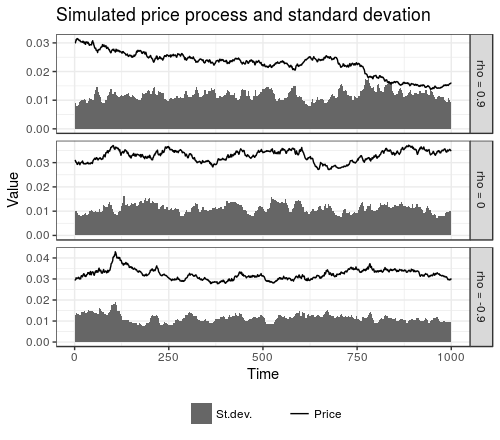
\includegraphics[width=\linewidth]{simulations/data-plot.pdf}
	\caption[Simulated price process and standard deviation]{Simulated price process scaled to 0.03 and its return's standard deviation. The relationship is visible: with high positive correlation (top) the price process and the volatility move together; with no correlation (middle) there is no visible pattern; with high negative correlation (bottom) the price process and the volatility move to the opposite direction.}
	\label{fig:simdata}
\end{figure}

\begin{figure}
	\centering
	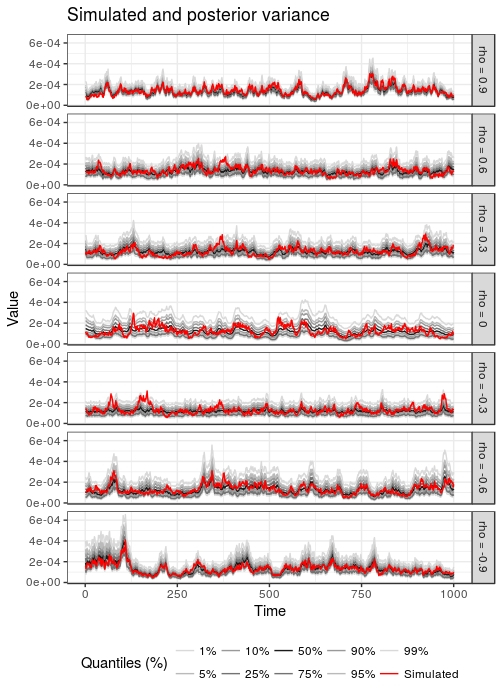
\includegraphics[width=\linewidth]{simulations/variance-plot.pdf}
	\caption{Simulated values and posterior quantiles of the variance process.}
	\label{fig:volatility}
\end{figure}

\begin{figure}
	\centering
	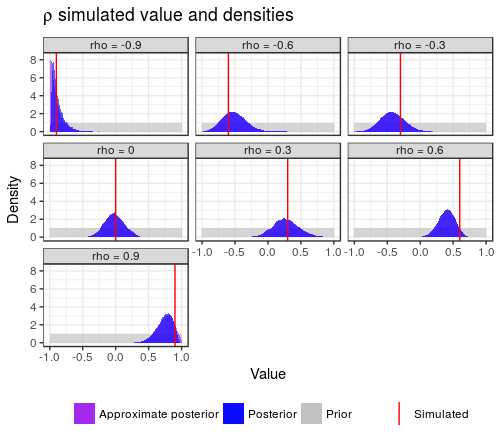
\includegraphics[width=\linewidth]{simulations/rho-densities.pdf}
	\caption[Prior, approximate and corrected posterior and simulated $\rho$]{Prior, approximate and corrected posterior distributions and the simulated value for $\rho$.}
	\label{fig:rhodensities}
\end{figure}
